\begin{exercício}{A resposta indutiva \enquote{perfeita}}{exercício5}
    Considere o arranjo mostrado na figura abaixo, onde há um campo magnético uniforme, perpendicular ao plano da figura, apenas na região hachurada.
    \begin{center}
        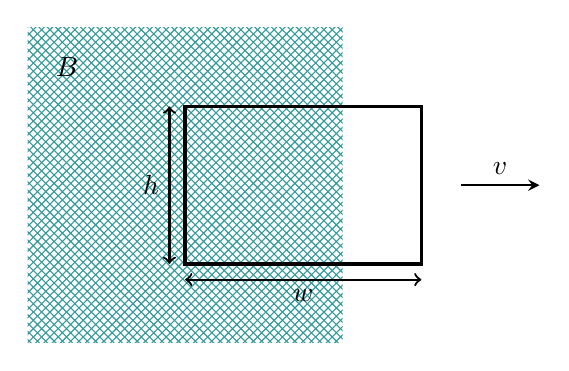
\begin{tikzpicture}
            \usetikzlibrary{patterns}
            \fill[pattern=crosshatch, pattern color=Teal!80] (0,0) rectangle (4,4);
            \node at (0.5,3.5) {\(\vetor{B}\)};
            \draw[very thick] (2,1) rectangle (5,3);
            \draw[thick, <->] (2,0.8) -- (5,0.8) node[midway,below] {\(w\)};
            \draw[thick, <->] (1.8,1) -- (1.8,3) node[midway,left] {\(h\)};
            \draw[-stealth, thick] (5.5,2) -- (6.5,2) node[midway,above] {\(\vetor{v}\)};
        \end{tikzpicture}
    \end{center}
    Suponha que a espira retangular, de lados \(h\) e \(w\), esteja se deslocando com uma velocidade constante \(\vetor{v}\), como indicado. Vimos em aula que a força eletromotriz total sobre o circuito da espira pode ser entendida como uma soma de dois termos,
    \begin{equation*}
        \varepsilon = \varepsilon_{\mathrm{fluxo}} + \varepsilon_{\mathrm{auto}} = - \diff{\Phi_{B}}{t} - L\diff{I}{t},
    \end{equation*}
    onde o primeiro termo diz respeito à variação do fluxo devido ao campo externo e o segundo à força eletromotriz induzida pela auto-indutância do próprio circuito, onde \(L\) é a auto-indutância da espira. Caso o fio tenha uma resistência interna \(R\), pode-se igualar \(\varepsilon = RI\) para obter uma equação diferencial para a função \(I(t)\). Contudo, caso possamos desprezar a resistência do fio, podemos igualar a força eletromotriz total a zero, significando que \(\varepsilon_{\mathrm{auto}} = -\varepsilon_{\mathrm{fluxo}}\). Nesse caso, calcule explicitamente \(\varepsilon_{\mathrm{fluxo}}\) em termos de \(\vetor{B}\), \(\vetor{v}\), \(h\), e do tempo \(t\), e encontre a corrente na espira \(I(t)\) para \(t > 0\). Considere que a espira começa a sair da região hachurada em \(t = 0\) e que \(I(0) = 0\). Faça um gráfico de \(I(t)\). Por fim, calcule a força magnética na espira devido ao campo externo em função do tempo.
\end{exercício}
\begin{proof}[Resolução]

\end{proof}
